\chapter{T\'{e}cnicas de segmentaci\'{o}n}

\section{Introducci\'{o}n}

Hay bastante controversia en cuanto a la clasificaci\'{o}n de las diferentes t\'{e}cnicas de segmentaci\'{o}n, por el gran n\'{u}mero de estas t\'{e}cnicas existentes, por las diferentes maneras en las que cada una tiene representada la imagen, las diferentes caracter\'{i}sticas que utilizan de la imagen etc. Hay trabajos que realizan una clasificaci\'{o}n de los algoritmos desde dos puntos de vista diferentes: en funci\'{o}n de c\'{o}mo puede ser utilizado el algoritmo, es decir, las aplicaciones que pueda tener, y otra en base al algoritmo en s\'{i}, fij\'{a}ndose en c\'{o}mo realiza la segmentaci\'{o}n \cite{mc1}. Por otro lado, tambi\'{e}n hay otros trabajos que realizan esta clasificaci\'{o}n para \'{a}mbitos muy concretos \cite[pag. 11]{mc1}.

\textit{Zhang}\cite{zhang1} propone una clasificaci\'{o}n m\'{a}s clara, creando la divisi\'{o}n en dos grupos: a) algoritmos basados en detectar la discontinuidad de las diferentes regiones de la imagen, los llamados \textit{edge-based algorithms} b) basados en detectar la continuidad o la similitud de las regiones, los llamados \textit{region-based algorithms}. Posteriormente hace una subdivisi\'{o}n de estos dos grupos en funci\'{o}n de la estrategia de procesamiento: los que realizan un procesamiento secuencial, donde el procesamiento de pasos previos se tienen en cuenta en pasos posteriores, y los que realizan un procesamiento paralelo, es decir, decisiones independientes y simult\'{a}neas \cite{zhang1}.

\begin{figure}[ht]
	\centering
	\captionsetup{justification=centering}
	\includegraphics[width=1\textwidth]{./imagenes/tecnicasSegmentacion2}
	\caption{Clasificaci\'{o}n de las t\'{e}cnicas de segmentaci\'{o}n}
	\vspace{2 mm}			
	Fuente: \cite{basa1}
	\label{tecnicasSegmentacion}
\end{figure}

La clasificaci\'{o}n elegida tiene varios aspectos en com\'{u}n con la \'{u}ltima presentada y descrita \cite{basa1}. Se ha preferido esta clasificaci\'{o}n al ser clara en cuanto a la divisi\'{o}n de las t\'{e}cnicas y las caracter\'{i}sticas que \'{e}stas tienen frente a otras clasificaciones. En la figura  \ref{tecnicasSegmentacion} se muestra el esquema de la clasificaci\'{o}n elegida.

\section{Segmentaci\'{o}n de imagen basada en el tratamiento de los \textit{p\'{i}xeles}}\label{cap:tratPixel}

Este tipo de segmentaci\'{o}n consiste en dividir la imagen en segmentos o  conjuntos de p\'{i}xeles (conocidos como <<superp\'{i}xeles>>). Cada p\'{i}xel de la imagen ser\'{a} tratado y agrupado en funci\'{o}n de sus caracter\'{i}sticas. Existen varios subgrupos dentro de esta clasificaci\'{o}n: \textit{Thresholding},o <<M\'{e}todo del valor umbral>> en castellano, y \textit{Clustering}, o algoritmos de agrupamiento en castellano, entre otros.

\subsection{Thresholding}

Este tipo de segmentaci\'{o}n es la m\'{a}s simple de todas y se basa en clasificar los p\'{i}xeles en dos grupos en funci\'{o}n de la intensidad de \'{e}stos: los que superan la intensidad umbral definida y los que no la superan. El resultado de esta segmentaci\'{o}n ser\'{i}a una imagen binaria (v\'{e}ase la comparaci\'{o}n de las figuras \ref{thresholding1} y \ref{thresholding2}). 

Esta t\'{e}cnica puede ser definida como:

\

Para una imagen NxM :

for $i = 1,2, ... , N \ $and$ \ j = 1,2, ... , M $
\begin{equation}
 f(n) = \left\{ 
\begin{array}{l l}
1 & \quad \mathrm{si \ I(i,j) \ge T}\\
0 & \quad \mathrm{si \ I(i,j) <\ T}
\end{array} \right. 
\end{equation}
donde $I(i,j)$ es el valor del p\'{i}xel de la posici\'{o}n i,j de la imagen.

Tambi\'{e}n existe la posibilidad de definir varias intensidades umbrales (v\'{e}ase la comparaci\'{o}n de las figuras \ref{thresholding3} y \ref{thresholding4}), con el fin de particionar la imagen en m\'{a}s segmentos. En s\'{i}, se podr\'{a}n definir tantos umbrales como niveles de gris contiene la imagen, aunque habr\'{a} que buscar un buen equilibrio. 

La ventaja de este tipo de segmentaci\'{o}n es que es relativamente sencilla comparada con otros tipos de segmentaci\'{o}n m\'{a}s avanzada como \textit{watershed} o \textit{level set}. Aun as\'{i}, esta segmentaci\'{o}n funciona bien cuando el fondo y los objetos siguen una distribuci\'{o}n bimodal, es decir, que hay una diferencia <<notable>> entre las dos partes. Com\'{u}nmente esta caracter\'{i}stica no se da en todas las im\'{a}genes, por lo que no tendr\'{a} buenos resultados en las que el fondo no se distinga bien de los objetos \cite{basa1}. Adem\'{a}s, esta segmentaci\'{o}n tampoco se comporta bien con im\'{a}genes que tienen una iluminaci\'{o}n gradiente grande (v\'{e}ase la comparaci\'{o}n de las figuras \ref{thresholding5} y \ref{thresholding6}). Aunque es verdad que para ello tambi\'{e}n existen varias mejoras que hacen que la segmentaci\'{o}n se <<adapte>> para conseguir mejores resultados.

En la figura \ref{tecnicasSegmentacion} se muestran varias subclases de \textit{thresholding}. Aunque no se explicar\'{a}n en profundidad conviene saber que hay varias maneras de realizar esta segmentaci\'{o}n. Primeramente se nombra el m\'{e}todo de Otso, \textit{Otsu's method} en ingl\'{e}s, que adapta el umbral en funci\'{o}n de la dispersi\'{o}n de los niveles de gris. El segundo m\'{e}todo, el \textit{Global}, es el m\'{a}s simple y el que hemos estado explicando hasta ahora. Y por \'{u}ltimo, el m\'{e}todo \textit{Adaptative}, mencionado anteriormente, que se adapta a la intensidad de la imagen.

\begin{figure}[H]
	\centering
	\captionsetup{justification=centering}
	\includegraphics[width=.65\textwidth]{./imagenes/imageHistogram}
	\caption{Histograma que muestra tres aparentes segmentos de la imagen con dos umbrales}
	\vspace{2 mm}					
	Fuente: \cite{basa1}	
	\label{imageHistogram}
\end{figure}

Las figuras \ref{thresHold1}, \ref{thresHold2} y \ref{thresHold3} muestran varios ejemplos de segmentaci\'{o}n utilizando \textit{thresholding}.
\vspace{-2 mm}			
\begin{figure}[H]
	\captionsetup{justification=centering}
	\centering
	\begin{subfigure}[t]{2.5in}
		\centering
		\includegraphics[width=.9\textwidth]{./imagenes/thresholding1}
		\subcaption{Imagen original}\label{thresholding1}		
	\end{subfigure}
	\begin{subfigure}[t]{2.5in}
		\centering
		\includegraphics[width=.9\textwidth]{./imagenes/thresholding2}
		\subcaption{Imagen segmentada}\label{thresholding2}
	\end{subfigure}
	\caption{Segmentaci\'{o}n con \textit{thresholding}}	
	\vspace{2 mm}			
	Fuente: commons.wikimedia.org	
	\label{thresHold1}
\end{figure}	
\begin{figure}[H]	
	\captionsetup{justification=centering}	
	\centering	
	\begin{subfigure}[t]{2.5in}
		\centering
		\includegraphics[width=.9\textwidth]{./imagenes/thresholding3}
		\subcaption{Imagen original}\label{thresholding3}
	\end{subfigure}
	\begin{subfigure}[t]{2.5in}
		\centering
		\includegraphics[width=.9\textwidth]{./imagenes/thresholding4}
		\subcaption{Imagen segmentada}\label{thresholding4}
	\end{subfigure}
	\caption{Segmentaci\'{o}n con \textit{thresholding} con varios umbrales}
	\vspace{2 mm}			
	Fuente: \textit{rosavallsformacio.tv} y \textit{photo-kako.com} para la realizaci\'{o}n de la segmentaci\'{o}n
	\label{thresHold2}
\end{figure}	
\begin{figure}[H]
	\centering
	\captionsetup{justification=centering}
	\begin{subfigure}[t]{2.5in}
		\centering
		\includegraphics[width=.7\textwidth]{./imagenes/thresholding5}
		\subcaption{Imagen original}\label{thresholding5}
	\end{subfigure}
	\begin{subfigure}[t]{2.5in}
		\centering
		\includegraphics[width=.7\textwidth]{./imagenes/thresholding6}
		\subcaption{Imagen segmentada}\label{thresholding6}
	\end{subfigure}
	\caption{Segmentaci\'{o}n con \textit{thresholding} en imagen con iluminaci\'{o}n gradiente}
	\vspace{2 mm}			
	Fuente: \textit{homepages.inf.ed.ac.uk/rbf/HIPR2/}
	\label{thresHold3}
\end{figure}


\subsection{Clustering}

Junto con la t\'{e}cnica de \textit{thresholding} el \textit{clustering} es la t\'{e}cnica de segmentaci\'{o}n m\'{a}s utilizada. En general esta t\'{e}cnica divide los puntos en varios \textit{clusters} o grupos en funci\'{o}n de la distancia entre ellos. En este caso concreto, los puntos ser\'{a}n los p\'{i}xeles de la imagen y la distancia entre ellos estar\'{a} relacionada con la intensidad, color y textura, pudiendo combinar varios de estos factores. 

Los algoritmos de \textit{clustering} se pueden dividir entre jer\'{a}rquicos y particionales, donde la principal diferencia entre los dos est\'{a} en el modo en que se construyen los grupos. Los algoritmos jer\'{a}rquicos suelen ser m\'{a}s precisos, sin embargo, no valen para una cantidad de datos grande como en una imagen ya que el coste computacional es muy elevado. Por lo tanto, la opci\'{o}n escogida suele ser el \textit{clustering} particional. No obstante, esta t\'{e}cnica tiene varias desventajas \cite{oli1}:

\begin{enumerate}
	\item Generalmente es necesario saber previamente el n\'{u}mero de \textit{clusters} que hay en la imagen. 
	\item No utilizan informaci\'{o}n espacial inherente a la imagen.
	\item En algunos algoritmos de clustering, como el K-means que se explicar\'{a} a continuaci\'{o}n, no se asegura un resultado \'{o}ptimo, ya que distintas inicializaciones dan diferentes resultados.
\end{enumerate} 

En la clasificaci\'{o}n presentada en la figura \ref{tecnicasSegmentacion} se muestran varias subclases de la t\'{e}cnica de \textit{clustering} que corresponden a diferentes algoritmos de creaci\'{o}n de \textit{clusters}. El algoritmo \textit{Fuzzy C-Means} agrupa los p\'{i}xeles utilizando la l\'{o}gica difusa, donde cada p\'{i}xel tendr\'{a} un grado de pertenencia a todos los \textit{clusters}. En general, hay muchos tipos de t\'{e}cnicas de clustering por lo que las t\'{e}cnicas restantes se agrupar\'{a}n en la secci\'{o}n de \textit{Others} de la figura \ref{tecnicasSegmentacion}. El algoritmo K-means es el m\'{a}s utilizado (v\'{e}ase ejemplos de su segmentaci\'{o}n en las figuras \ref{clusteringTotal1} y \ref{clusteringTotal2}). Una descripci\'{o}n de su modo de funcionamiento a grandes rasgos ser\'{i}a:

\begin{enumerate}
 \item Se asignan \textit{K} primeros p\'{i}xeles como centroides.
 \item Se agrupan los p\'{i}xeles, restantes con los centroides definidos en funci\'{o}n de la distancia con estos.
 \item Se calculan los nuevos \textit{K} centroides como los baricentros de los \textit{K} conglomerados obtenidos.
 \item Se alternan los pasos 2 y 3 hasta que se alcance un determinado criterio de convergencia (m\'{a}xima variaci\'{o}n de centroides, por ejemplo).
\end{enumerate}

\begin{figure}[H]
	\captionsetup{justification=centering}
	\centering
	\begin{subfigure}[t]{2.5in}
		\centering
		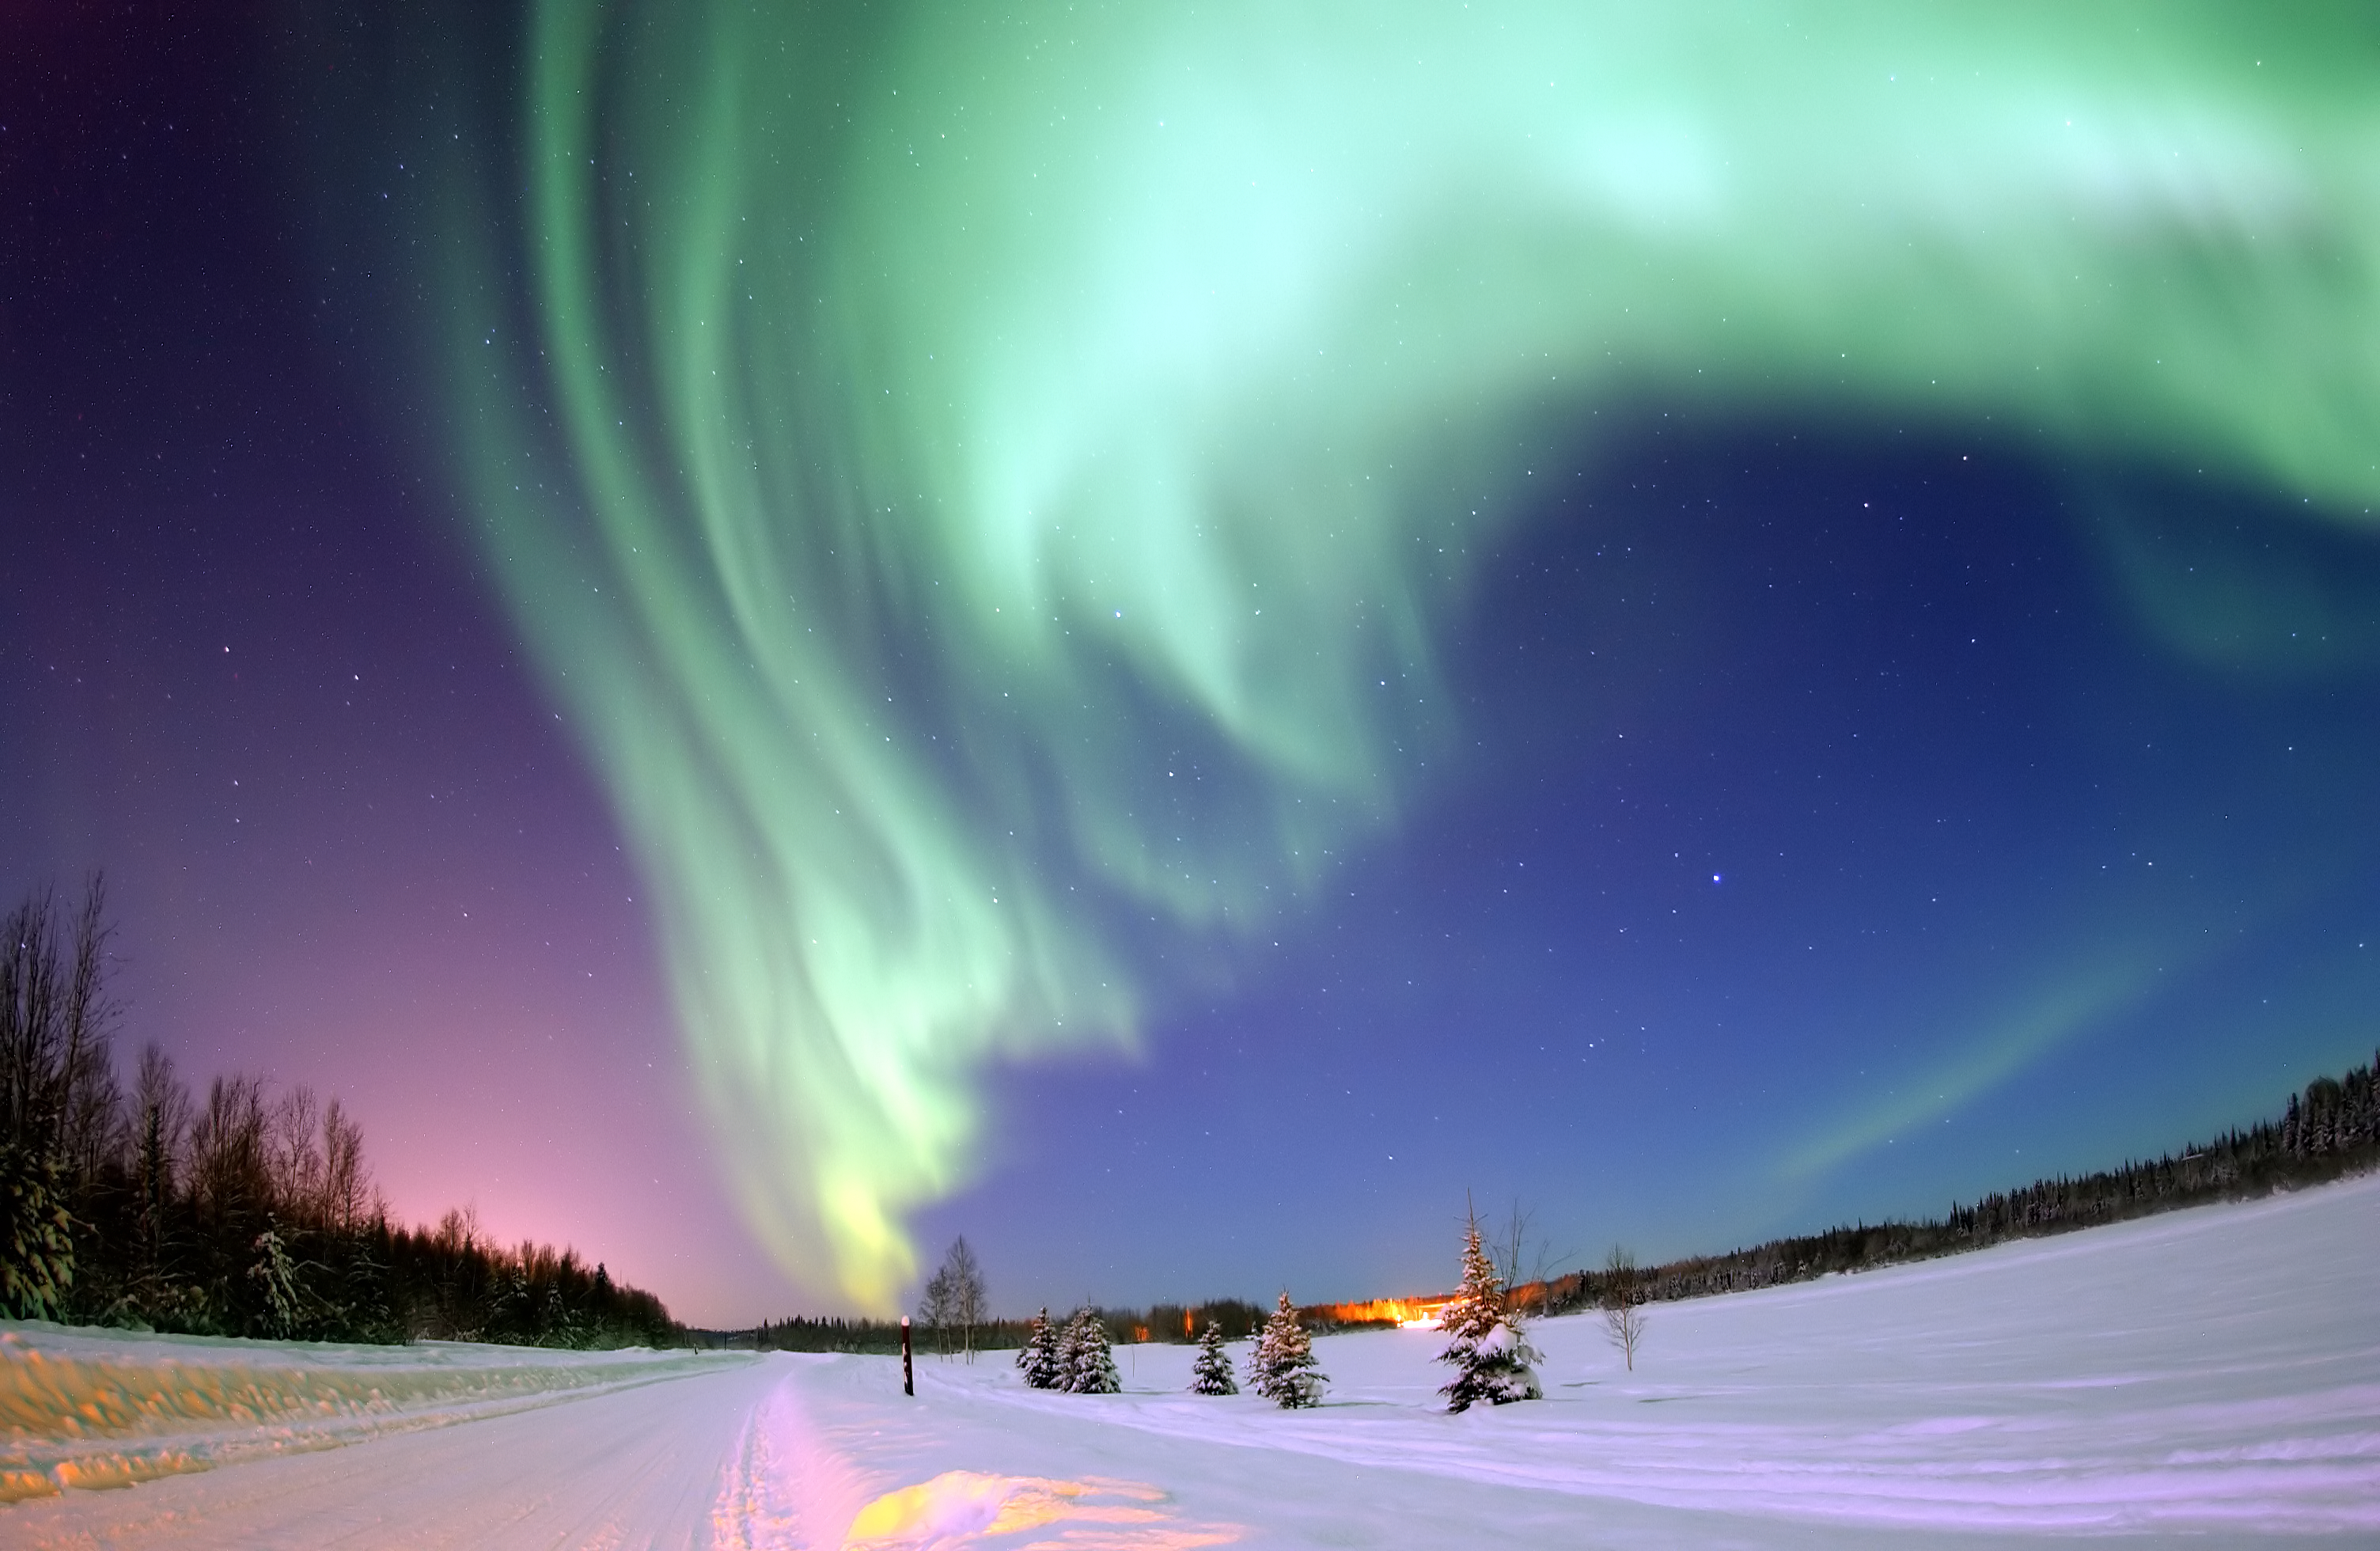
\includegraphics[width=.9\textwidth]{./imagenes/clustering1}
		\subcaption{Imagen original}\label{clustering1}
	\end{subfigure}
	\begin{subfigure}[t]{2.5in}
		\centering
		\includegraphics[width=.9\textwidth]{./imagenes/clustering2}
		\subcaption{Imagen segmentada}\label{clustering2}
	\end{subfigure}
	\caption{Segmentaci\'{o}n utilizando K-means con K=16}
	\vspace{2 mm}
	\label{clusteringTotal1}			
	Fuente: commons.wikipedia.org
\end{figure}
\begin{figure}[H]
	\centering
	\captionsetup{justification=centering}
	\begin{subfigure}[t]{2.5in}
		\centering
		\includegraphics[width=1\textwidth]{./imagenes/clustering3}
		\subcaption{Imagen original}\label{clustering3}
	\end{subfigure}
	\begin{subfigure}[t]{2.5in}
		\centering
		\includegraphics[width=1\textwidth]{./imagenes/clustering4}
		\subcaption{Imagen segmentada}\label{clustering4}
	\end{subfigure}
	\caption{Segmentaci\'{o}n utilizando K-means con K=6}
	\vspace{2 mm}
	\label{clusteringTotal2}			
	Fuente: \textit{imagedatabase.cs.washington.edu/demo/kmcluster/}
\end{figure}

\subsection{Morphology}

La t\'{e}cnica de la morfolog\'{i}a, o \textit{morphology} en ingl\'{e}s, se clasificar\'{i}a dentro de las t\'{e}cnicas basadas en el tratamiento de los p\'{i}xeles. Hay varios m\'{e}todos de morfolog\'{i}a y se basan en una m\'{a}scara llamada \textit{structuring element} para investigar cada p\'{i}xel. El valor de cada p\'{i}xel est\'{a} determinado por el de sus vecinos que pertenecen a esa m\'{a}scara. Los m\'{e}todos m\'{a}s simples de esta t\'{e}cnica son la dilataci\'{o}n y la erosi\'{o}n. Para una imagen binaria, la dilataci\'{o}n convierte en uno todos los p\'{i}xeles de la m\'{a}scara si los p\'{i}xeles <<debajo>> del p\'{i}xel central son ceros como se muestra en la imagen \ref{morphology1}. La erosi\'{o}n es el caso contrario, es decir, convierte en ceros todos los elementos de la m\'{a}scara si esta contiene alg\'{u}n elemento que sea cero. La combinaci\'{o}n de estas simples operaciones junto con otras como el complemento, la uni\'{o}n y la intersecci\'{o}n, pueden utilizarse para realizar operaciones m\'{a}s avanzadas y complejas. 
 
\begin{figure}[ht]
	\centering
	\captionsetup{justification=centering}
	\begin{subfigure}[t]{2.5in}
		\centering
		\includegraphics[width=.8\textwidth]{./imagenes/morphology1-1}
		\subcaption{Imagen sin tratar}\label{morphology1.1}
	\end{subfigure}	
	\begin{subfigure}[t]{2.5in}
		\centering
		\includegraphics[width=.8\textwidth]{./imagenes/morphology1-2}
		\subcaption{Resultado de la dilataci\'{o}n}\label{morphology1.2}
	\end{subfigure}
	\caption{Ejemplo de dilataci\'{o}n de la t\'{e}cnica de morfolog\'{i}a}
	\vspace{2 mm}
	Fuente: \cite{eri2015}
	\label{morphology1}
\end{figure}

\section{Segmentaci\'{o}n de imagen basada en la detecci\'{o}n de bordes}

Este tipo de segmentaci\'{o}n consiste en encontrar los bordes de los objetos contenidos en la imagen con el fin de poder dividir la imagen en funci\'{o}n de los bordes encontrados. Los detectores de bordes tradicionales suelen utilizar los operadores diferenciales de detecci\'{o}n de bordes comentados en \ref{cap:EvoSeg}, es decir, los operadores \textit{Sobel}, \textit{Roberts} y \textit{Prewitt edge detectors} que est\'{a}n basados en el gradiente de la funci\'{o}n de intensidad de una imagen. Normalmente los bordes suelen detectarse en las intersecciones de dos regiones de la imagen que tienen diferentes intensidades.

La ventaja de este tipo de segmentaci\'{o}n frente a la basada en el tratamiento de p\'{i}xeles es que, aparte de hacer la divisi\'{o}n de las diferentes regiones, sabremos exactamente d\'{o}nde se encuentran los bordes de \'{e}stas, siendo \'{u}til para poder extraerlas y poder tratarlas individualmente. Por lo tanto, esta t\'{e}cnica funcionar\'{a} mejor cuando la diferencia entre las regiones tenga buena calidad. Una de las posibles <<desventajas>> puede ser que la detecci\'{o}n de muchos bordes dificulte la extracci\'{o}n de las regiones de inter\'{e}s.

Existen varios subgrupos dentro de esta clasificaci\'{o}n: \textit{Edge detection} o <<Detecci\'{o}n de bordes>> en castellano, t\'{e}cnicas que tienen que ver con el gradiente de la imagen \textit{Gradient mode}, \textit{Active contours} o <<Contornos activos>> y \textit{level sets} o t\'{e}cnicas del <<Conjunto de nivel>>.

\subsection{Detecci\'{o}n de borde usando gradientes}

En la figura \ref{tecnicasSegmentacion} se diferencian las dos primeras clasificaciones \textit{Edge detection} y \textit{Gradient mode} pero al estar directamente relacionadas se ha decidido explicarlas en conjunto. 

Las t\'{e}cnicas cl\'{a}sicas de detecci\'{o}n de bordes se basan en encontrar la derivada respecto a los ejes que forman la imagen, o dicho de otro modo, el gradiente. El gradiente de un punto de una funci\'{o}n escalar, representado con $\nabla$, se representa en forma vectorial. Este vector indica la direcci\'{o}n en la cual la funci\'{o}n varia m\'{a}s r\'{a}pidamente y su m\'{o}dulo representa el ritmo de variaci\'{o}n de la funci\'{o}n en la direcci\'{o}n de dicho vector. Este m\'{o}dulo se utilizar\'{a} para determinar si un punto es borde o no, en funci\'{o}n de si supera un valor umbral dado. Para encontrar la m\'{a}xima variaci\'{o}n en ese punto se deben de hacer las derivadas parciales respecto a cada eje y coger el m\'{a}ximo valor de \'{e}stas. En general el gradiente se suele aproximar con la f\'{o}rmula\protect\footnotemark \footnotetext{V\'{a}lida para una imagen de dos dimensiones. En caso de tener tres dimensiones la f\'{o}rmula ser\'{i}a $|G| \approx |G_x| + |G_y| + |G_z| $ }$|G| \approx |G_x| + |G_y| $  que es mucho m\'{a}s simple de implementar en la pr\'{a}ctica. Vali\'{e}ndonos de esto, se desarrollaron los primeros operadores diferenciales ya comentados  \textit{Sobel}, \textit{Roberts} y \textit{Prewitt edge detectors} (v\'{e}ase un ejemplo de cada segmentaci\'{o}n en la figura \ref{prewittTable2}). Estos operadores no son m\'{a}s que m\'{a}scaras aplicadas al p\'{i}xel a tratar y a cierta vecindad de \'{e}ste para calcular una aproximaci\'{o}n a dichas derivadas $G_x$ y $G_y$. De ah\'{i} el nombrarlos como <<operadores>>.

\

\subsubsection{$\blacksquare$ \quad Roberts operator}

Este operador es el m\'{a}s simple de los tres mencionados y aproxima las derivadas tomando la diferencia de dos valores contiguos. La gran desventaja de este operador es que es muy sensible al ruido al tratar pocos vecinos y s\'{o}lo permite marcar los puntos del borde pero no su orientaci\'{o}n. A pesar de todo ello, es un operador que computacionalmente es poco costoso debido a su simpleza y que trabaja bien con im\'{a}genes binarias. V\'{e}ase las m\'{a}scaras utilizadas por esta t\'{e}cnica presentada en la tabla \ref{robetsTable}. 

\begin{table}[H]
	\parbox{.65\linewidth}{
		\centering
		\begin{tabular}{|c|c|}
			\hline
			+1 & 0 \\ \hline
			0  & -1 \\ \hline
		\end{tabular}
		\caption*{$G_x$}
	}
	\hspace*{-50mm}
	\parbox{.65\linewidth}{
		\centering
		\begin{tabular}{|c|c|}
			\hline
			0 & +1 \\ \hline
			-1  & 0 \\ \hline
		\end{tabular}
		\caption*{$G_y$}
	}
	\captionsetup{justification=centering}
	\caption{M\'{a}scaras utilizadas por el operador de Roberts de tama\~{n}o 2x2}
	\label{robetsTable}
\end{table}

\subsubsection{$\blacksquare$ \quad Sobel operator}

Este operador utiliza una m\'{a}scara m\'{a}s grande que el \textit{Roberts operator}, 3x3, por lo que implicar\'{a} a m\'{a}s vecinos. Enfatiza m\'{a}s los p\'{i}xeles de alrededor del centro. La ventaja de este operador es que es menos sensible al ruido, detecta muy bien los bordes horizontales y verticales y adem\'{a}s proporciona un suavizado. Las desventaja de este operador es que computacionalmente es m\'{a}s costoso, no tiene buena detecci\'{o}n de bordes diagonales y no da informaci\'{o}n sobre la orientaci\'{o}n del borde. V\'{e}ase las m\'{a}scaras utilizadas por esta t\'{e}cnica presentada en la tabla \ref{sobelTable}.
\begin{table}[H]
	\parbox{.45\linewidth}{
	\centering
		\begin{tabular}{|c|c|c|}
			\hline
			-1 & 0 & +1 \\ \hline
			-2 & 0 & +2 \\ \hline
			-1 & 0 & +1 \\ \hline
		\end{tabular}
	\caption*{$G_x$}
	}
	\parbox{.45\linewidth}{
	\centering
		\begin{tabular}{|c|c|c|}
			\hline
			+1 & +2 & +1 \\ \hline
			0  & 0  & 0  \\ \hline
			-1 & -2 & -1 \\ \hline
		\end{tabular}
		\caption*{$G_y$}
	}
	\captionsetup{justification=centering}
	\caption{M\'{a}scaras utilizadas por el operador de Sobel de tama\~{n}o 3x3}
	\label{sobelTable}
\end{table}

\subsubsection{$\blacksquare$ \quad Prewitt operator}

Este operador es parecido al operador de Sobel pero este no enfatiza los p\'{i}xeles cercanos al centro y los coeficientes son diferentes. Las ventajas son que aumenta la respuesta a los bordes diagonales poni\'{e}ndole peso a p\'{i}xeles vecinos que antes no ten\'{i}an, tiene poca sensibilidad la ruido y proporciona la magnitud y orientaci\'{o}n del borde (hasta 8 direcciones). V\'{e}ase las m\'{a}scaras utilizadas por esta t\'{e}cnica presentada en las tablas \ref{prewittTable1} y \ref{prewittTable2}.
 \begin{table}[H]
 	\parbox{.45\linewidth}{
 		\centering
		\begin{tabular}{|c|c|c|}
			\hline
			-1 & +1 & +1 \\ \hline
			-1 & -2 & +2 \\ \hline
			-1 & +1 & +1 \\ \hline
		\end{tabular}
 		\caption*{0}
 	}
 	\parbox{.45\linewidth}{
 		\centering
			\begin{tabular}{|c|c|c|}
				\hline
				+1 & +1 & +1 \\ \hline
				-1 & -2 & +1 \\ \hline
				-1 & +1 & +1 \\ \hline
			\end{tabular}
 		\caption*{45}
 	}
	\captionsetup{justification=centering}
 	\caption{M\'{a}scaras utilizadas por el operador de Prewitt de tama\~{n}o 3x3}
	\label{prewittTable1}
 \end{table}

\begin{figure}[H]
	\captionsetup{justification=centering}
	\begin{subfigure}[t]{2.5in}
		\centering
		\includegraphics[width=.9\textwidth]{./imagenes/operator0}
		\subcaption{Imagen original}\label{operator0}
	\end{subfigure}
	\begin{subfigure}[t]{2.5in}
		\centering
		\includegraphics[width=.9\textwidth]{./imagenes/operator1}
		\subcaption{Resultado de \textit{Roberts operator}}\label{operator1}
	\end{subfigure}
	
	\begin{subfigure}[t]{2.5in}
		\centering
		\includegraphics[width=.9\textwidth]{./imagenes/operator2}
		\subcaption{Resultado de \textit{Sovel operator}}\label{operator2}
	\end{subfigure}
	\begin{subfigure}[t]{2.5in}
		\centering
		\includegraphics[width=.9\textwidth]{./imagenes/operator3}
		\subcaption{Resultado de \textit{Prewitt operator}}\label{operator3}
	\end{subfigure}
	\caption{Detecci\'{o}n de bordes con el uso de los operadores}
	\vspace{2 mm}
	\centering
	\label{prewittTable2}
	Fuente: commons.wikipedia.org
\end{figure}

\subsection{Active Contours}\label{cap:actContour}

Desde que fueron introducidos por Kass y colaboradores en 1988 \cite{kass1}, los contornos activos o m\'{a}s com\'{u}nmente nombrados como \textit{Snakes}, han ganado popularidad gracias a los buenos resultados que se pueden llegar a obtener en la segmentaci\'{o}n de im\'{a}genes. 

Un contorno activo o \textit{Snake} es una curva el\'{a}stica que comienza a moverse dada una posici\'{o}n inicial de manera que llegue a delimitar las regiones de inter\'{e}s de la imagen. La curva se ir\'{a} moviendo de manera que se minimice su energ\'{i}a hasta llegar a un punto de convergencia. El contorno puede ser definido param\'{e}tricamente como $V(s) = [x(s),y(s)]$ donde $x(s)$ e $y(s)$ son las coordenadas de la parte $s$ del contorno. La energ\'{i}a del contorno est\'{a} compuesta por una energ\'{i}a interna y otra externa, $E_{int}$ y $E_{ext}$ respectivamente. La definici\'{o}n formal ser\'{i}a:

\begin{equation}
E = \int_{0}^{1}E_{int}(v,s) + E_{ext}(v(s)) ds
\end{equation}

$E_{int}$ da las caracter\'{i}sticas de deformaci\'{o}n del contorno el\'{a}stico, por lo tanto depende de la forma que \'{e}ste tenga. La $E_{int}$ puede ser definida como:
\begin{equation}
E_{int} = \frac{1}{2} (\alpha|\frac{\delta v}{\delta s}|^2 + \beta|\frac{\delta^2 v}{\delta s^2}| ^2)
\end{equation}
y los valores $\alpha$ y $\beta$ determinan el grado en el que el contorno se puede estirar o curvar. Un aumento en la magnitud $\alpha$ incrementar\'{i}a la tensi\'{o}n de la curva y un aumento de $\beta$ incrementar\'{i}a la rigidez de la curva, haciendo que sea menos flexible.

En cuanto a la energ\'{i}a externa hay varias maneras de definirla. Una elecci\'{o}n popular ser\'{i}a la magnitud negativa del gradiente de la imagen que se definir\'{i}a como:
\begin{equation}
E_{int}(\vec{x}) = - |\nabla [G_{\alpha} I(\vec{x})]|^2
\end{equation}
donde $G_{\alpha}$ es una convoluci\'{o}n con un filtro pasa bajo gaussiano. Esta propuesta de energ\'{i}a hace que el contorno se expanda hasta los bordes que haya en la imagen como se puede ver en la figura \ref{activeContour1}.
\begin{figure}[H]
	\captionsetup{justification=centering}
	\centering
	\begin{subfigure}[t]{2.5in}
		\centering
		\includegraphics[width=.9\textwidth]{./imagenes/activeContour1-1}
		\subcaption{}\label{activeContour1.1}
	\end{subfigure}
	\begin{subfigure}[t]{2.5in}
		\centering
		\includegraphics[width=.9\textwidth]{./imagenes/activeContour1-2}
		\subcaption{}\label{activeContour1.2}
	\end{subfigure}
	\caption{Ejemplo de un contorno activo}
	\vspace{2 mm}
	Fuente: \cite{eri2015}
	\label{activeContour1}
\end{figure}

La imagen \ref{activeContour1.1} corresponde a la imagen de entrada, mientras que la imagen \ref{activeContour1.2} corresponde a la convoluci\'{o}n de la magnitud gradiente de la imagen de entrada con un filtro pasa bajo gaussiano. La l\'{i}nea interior (roja) en la imagen \ref{activeContour1.2} es el contorno activo que se mover\'{a} hasta la l\'{i}nea exterior (verde) que corresponde con el borde de la imagen original. Un ejemplo de la aplicaci\'{o}n de esta t\'{e}cnica se puede ver en la figura \ref{activeContour2}.

\begin{figure}[H]
	\captionsetup{justification=centering}	
	\centering
	\includegraphics[width=.8\textwidth]{./imagenes/activeContour2}
	\caption{Ejemplo de segmentaci\'{o}n de plantas presentando en \cite{suta1} utilizando los contornos activos}
	\vspace{2 mm}
	Fuente: \cite{suta1}	
	\label{activeContour2}
\end{figure}


\subsection{\textit{Level set}}\label{levelSet}
Conjuntos de nivel, o \textit{level set} en ingl\'{e}s, es un tipo de segmentaci\'{o}n muy parecida a la que hemos explicado en la secci\'{o}n \ref{cap:actContour} ya que tambi\'{e}n se trata de expandir un contorno dado previamente para encontrar los bordes de la imagen. La ventaja de este m\'{e}todo frente al referido es que permite juntar y dividir contornos sin ning\'{u}n c\'{a}lculo extra necesario.

El contorno est\'{a} representado por la funci\'{o}n de \textit{level set}, que est\'{a} definida en una dimensi\'{o}n m\'{a}s que las dimensiones de la imagen a segmentar, es decir, para una imagen 2D tendr\'{i}amos una superficie de \textit{level set} de tres dimensiones mientras que para una imagen de 3D tendr\'{i}amos una superficie de 4D. En el caso de una superficie de 3D \'{e}sta tiene una forma c\'{o}nica como se puede ver en la figura \ref{levelSet1}. Suponiendo entonces que la imagen a tratar tiene dos dimensiones, podr\'{i}amos definir la funci\'{o}n de \textit{level set} como $z = \phi(x,y,t)$ que devuelve la altura de la superficie de \textit{level set} en el punto $(x,y)$ del plano de la imagen en el tiempo $t$. El contorno es definido impl\'{i}citamente como <<zero \textit{level set}>>, donde la altura del plano respecto a la superficie es cero ($\phi(x,y,t) = 0$). Esto es justo la intersecci\'{o}n entre el plano de la imagen y la superficie. V\'{e}ase las figuras \ref{levelSet1} y \ref{levelSet2} para ver ilustraciones de la t\'{e}cnica \textit{level set}.

\

Para propagar el contorno se mueve la superficie de \textit{level set} en el eje z, como se puede ver en la figura \ref{levelSet1}. La rapidez y la direcci\'{o}n en la que se mueve el contorno est\'{a} determinada por como se curva la superficie de \textit{level set}. Suponiendo que cada punto del contorno se mueve en una direcci\'{o}n ortogonal frente al contorno con una velocidad F, el contorno evoluciona usando la siguiente PDE (\textit{partial differential equation} o ecuaci\'{o}n en derivadas parciales en castellano):

\begin{equation}
\frac{\delta \phi(x,y,t)}{\delta t} = F(x,y,I) |\nabla \phi(x,y,t)|
\end{equation}

Esta funci\'{o}n de velocidad var\'{i}a dependiendo del punto de la imagen I a tratar y hace que el contorno se expanda a ciertas \'{a}reas de la imagen y no lo haga en otras zonas de esta. Normalmente la funci\'{o}n de velocidad se define por la intensidad o el gradiente de los p\'{i}xeles y por la curva de la funci\'{o}n de \textit{level set}.

De la idea de que modificaciones de p\'{i}xeles lejanos al contorno no afectan a este surgen varias mejoras de esta t\'{e}cnica que tienen en cuenta los p\'{i}xeles con los que se trabajar\'{a} en cada iteraci\'{o}n: \textit{narrow band} y \textit{sparse field methods}. El m\'{e}todo de \textit{narrow band} actualiza los p\'{i}xeles en una l\'{i}nea estrecha alrededor del contorno. El m\'{e}todo \textit{sparse field} actualiza los p\'{i}xeles vecinos del contorno \'{u}nicamente.

\begin{figure}[H]
	\captionsetup{justification=centering}
	\centering
	\includegraphics[width=.7\textwidth]{./imagenes/levelSet1}
	\caption{Ilustraci\'{o}n de la superficie de \textit{level set}}
	\vspace{2 mm}
	Fuente: \cite{eri2015}
	\label{levelSet1}
\end{figure}
\

\

\

\

\begin{figure}[H]
	\captionsetup{justification=centering}
	\centering
	\includegraphics[width=.7\textwidth]{./imagenes/levelSet2}
	\caption{Ilustraci\'{o}n del m\'{e}todo \textit{level set}}
	\vspace{2 mm}
	Fuente: commons.wikipedia.org
	\label{levelSet2}
\end{figure}

\section{Segmentaci\'{o}n de imagen basada en regiones crecientes}\label{cap:segRegiCreci}

Este tipo de segmentaci\'{o}n, m\'{a}s conocida como \textit{region growing}, se basa en la idea de que los p\'{i}xeles de una regi\'{o}n tienen caracter\'{i}sticas comunes, como puede ser, la intensidad de gris etc. Por ello, al tener que tratar un nuevo p\'{i}xel si este tiene una intensidad de gris parecida a la intensidad de grises que contiene la regi\'{o}n significar\'{a} que ese punto pertenece a ella. 

Existen varios subgrupos dentro de esta clasificaci\'{o}n: t\'{e}cnicas basadas en la idea de regiones crecientes, o \textit{region growing} en ingl\'{e}s, t\'{e}cnicas de \textit{Split/Merge} y t\'{e}cnicas basadas en grafos \textit{Graphs cuts}.

\subsection{\textit{Region growing}}

Este subgrupo agrupa todos las t\'{e}cnicas que siguen la idea de agrupar los p\'{i}xeles con caracter\'{i}sticas comunes, como el nivel de gris o el color de \'{e}stos. Hay dos t\'{e}cnicas conocidas que siguen esta metodolog\'{i}a, por lo que en esta ocasi\'{o}n explicaremos m\'{a}s de una t\'{e}cnica de este subgrupo de segmentaci\'{o}n.

\subsubsection{$\blacksquare$ \quad \textit{Region growing} o \textit{Seeded-based region growing segmentation}}

Este tipo de segmentaci\'{o}n comienza con la selecci\'{o}n de un p\'{i}xel, denominado a menudo como semilla o \textit{seed} en ingl\'{e}s, que est\'{a} dentro del objeto de inter\'{e}s. Normalmente la semilla se elige manualmente. A partir de ese p\'{i}xel semilla (primer punto de la regi\'{o}n) se comenzar\'{a} a extender la regi\'{o}n procesando sus vecinos y a\~{n}adi\'{e}ndolos en base a un criterio predefinido. Este criterio de inserci\'{o}n ser\'{a} en base a la intensidad, color o textura de la semilla y los puntos que pertenezcan a la regi\'{o}n. Cada vez que se inserta un nuevo punto a la regi\'{o}n la caracter\'{i}stica que se est\'{e} utilizando para realizar la inserci\'{o}n se volver\'{a} a calcular, por ejemplo, si se utiliza el nivel de gris, se volver\'{a} a calcular el valor medio de los niveles de gris que hay en la regi\'{o}n generada hasta el momento. De esta manera, la regi\'{o}n se ir\'{a} expandiendo a\~{n}adiendo vecinos hasta que encuentre alguno que no cumpla con la condici\'{o}n de inserci\'{o}n impuesta por el criterio. Si un punto no ha sido a\~{n}adido a ninguna regi\'{o}n se podr\'{a} a\~{n}adir a una regi\'{o}n cercana suya si la diferencia entre, por ejemplo, el nivel de gris de este punto y el nivel de gris medio de la regi\'{o}n no supera un valor umbral \textit{T} dado. V\'{e}ase un ejemplo de esta t\'{e}cnica en la figura \ref{regionGrowing1}.

Esta t\'{e}cnica es \'{u}til cuando la intensidad del fondo y del objeto son muy parecidas pero est\'{a}n separadas por un borde <<notable>> o por otra regi\'{o}n.
\begin{figure}[H]
	\captionsetup{justification=centering}
	\centering
	\includegraphics[width=.4\textwidth]{./imagenes/regionGrowing1}
	\caption{Ejemplo del funcionamiento de la t\'{e}cnica de \textit{region growing}}
	\vspace{2 mm}
	Fuente: \cite{eri2015}
	\label{regionGrowing1}
\end{figure}
\

\

\

\begin{figure}[H]
	\captionsetup{justification=centering}
	\begin{center}
		\begin{subfigure}[t]{2.5in}
			\centering
			\includegraphics[width=.9\textwidth]{./imagenes/regionGrowing6}
			\subcaption{Imagen original}\label{regionGrowing6}
		\end{subfigure}
	\end{center}	
	\begin{subfigure}[t]{2.5in}
		\centering
		\includegraphics[width=.9\textwidth]{./imagenes/regionGrowing2}
		\subcaption{\textit{Region growing} con un valor umbral T=255}\label{regionGrowing2}
	\end{subfigure}
	\begin{subfigure}[t]{2.5in}
		\centering
		\includegraphics[width=.9\textwidth]{./imagenes/regionGrowing3}
		\subcaption{\textit{Region growing} con un valor umbral T=225}\label{regionGrowing3}
	\end{subfigure}	
	\begin{subfigure}[t]{2.5in}
		\centering
		\includegraphics[width=.9\textwidth]{./imagenes/regionGrowing4}
		\subcaption{\textit{Region growing} con un valor umbral T=190}\label{regionGrowing4}
	\end{subfigure}
	\begin{subfigure}[t]{2.5in}
		\centering
		\includegraphics[width=.9\textwidth]{./imagenes/regionGrowing5}
		\subcaption{\textit{Region growing} con un valor umbral T=155}\label{regionGrowing5}
	\end{subfigure}
	\caption{Ejemplo de la t\'{e}cnica de \textit{region growing}}
	\centering
	\vspace{2 mm}
	\label{regionGrowingEntera}
	Fuente: commons.wikipedia.org
\end{figure}

En la figura \ref{regionGrowingEntera} se puede ver un ejemplo de la t\'{e}cnica de \textit{region growing} donde se quiere encontrar la parte del rayo m\'{a}s fuerte en la imagen. Para ello se eligen como semilla los puntos con mayor valor de gris posible(255). El criterio de inserci\'{o}n de los p\'{i}xeles es tener el "mismo" nivel de gris. En este caso se ha decidido que los puntos que no han sido insertados en una regi\'{o}n se inserten en una cercana si superan el valor umbral \textit{T} dado. Por ello en \ref{regionGrowing2} solo aparecen los puntos semilla ya que no se habr\'{a}n unido puntos con este criterio y el valor \textit{T} es demasiado alto. En las im\'{a}genes \ref{regionGrowing3}, \ref{regionGrowing4} y \ref{regionGrowing5} ese valor \textit{T} se va disminuyendo y cada vez se insertan m\'{a}s puntos en la regi\'{o}n. 

\

\

\subsubsection{$\blacksquare$ \quad \textit{Watershed}}

La idea principal de esta t\'{e}cnica se basa en ver la imagen como una imagen tridimensional donde la tercera dimensi\'{o}n es la altura del p\'{i}xel. La altura del p\'{i}xel est\'{a} determinada por su nivel de gris. Topol\'{o}gicamente quedar\'{a} algo como se puede ver en \ref{watershed1}. En este <<terreno>> creado se podr\'{a}n diferenciar hasta tres puntos. Estos puntos son determinados con la analog\'{i}a de como una gota de agua caer\'{i}a y se mover\'{i}a si se precipitase en ese punto. Hay tres tipos de puntos:
\begin{enumerate}
	\item Puntos con un nivel de gris m\'{i}nimo local donde la gota se estancar\'{i}a.
	\item Puntos en los que la gota caer\'{i}a o se deslizar\'{i}a hacia un \'{u}nico punto m\'{i}nimo local.
	\item Puntos en los que la gota podr\'{i}a caer hacia m\'{a}s de un punto m\'{i}nimo local.
\end{enumerate}
El segundo tipo de puntos son nombrados como \textit{watershed} ,o cuencas en castellano, y los del tercer tipo son nombrados como \textit{watersheds lines}, bordes o l\'{i}neas de las cuencas en castellano.

El objetivo final de esta t\'{e}cnica ser\'{a} encontrar los bordes de las cuencas, que representar\'{a}n los bordes de la imagen original. Para ello existen varias maneras de hacerlo, la m\'{a}s com\'{u}n es la t\'{e}cnica de \textit{flooding}. La idea es simple, imaginemos que se empieza a echar agua en los puntos de tipo uno, es decir, los que representan un m\'{i}nimo local y son <<cuencas>>. El nivel del agua empezar\'{a} a subir hasta que llegue a un punto en el que la cuenca se empiece a desbordar y vaya a juntarse con otra cuenca. En ese momento, se construye una presa o un muro de manera que el agua no se desborde. Esas presas o muros construidos ser\'{a}n los bordes de las cuencas. Con todas estas presas se habr\'{a} conseguido la segmentaci\'{o}n de la imagen.

\begin{figure}[H]
	\captionsetup{justification=centering}
	\centering
	\includegraphics[width=.7\textwidth]{./imagenes/watershed1}
	\caption{Ejemplo del funcionamiento de la t\'{e}cnica de \textit{watershed}}
	\vspace{2 mm}
	Fuente: \cite{eri2015}
	\label{watershed1}
\end{figure}
En la figura \ref{watershed2} se puede ver el un ejemplo del funcionamiento de la t\'{e}cnica de \textit{watershed} donde la intensidad de los p\'{i}xeles de la imagen de la izquierda ser\'{a}n la altura de ese mismo punto en la imagen derecha, creando as\'{i} ese terreno.

\begin{figure}[H]
	\captionsetup{justification=centering}
	\centering
	\includegraphics[width=.8\textwidth]{./imagenes/watershed2}
	\caption{Funcionamiento de la t\'{e}cnica de \textit{watershed}}
	\vspace{2 mm}	
	Fuente: \textit{http://www.di.ubi.pt/$\sim$agomes/cvm/teoricas/07-regionsegmentation.pdf}	
	\label{watershed2}
\end{figure}

En la figura \ref{watershed3} se muestra el funcionamiento de la t\'{e}cnica de \textit{watershed} donde se puede ver como va creciendo el nivel de agua hasta encontrar ese <<punto>> de desbordamiento en el que se marcan los bordes.

\begin{figure}[H]
	\captionsetup{justification=centering}
	\centering
	\includegraphics[width=.6\textwidth]{./imagenes/watershed3}
	\caption{Funcionamiento de la t\'{e}cnica de \textit{watershed}}
	\vspace{2 mm}		
	Fuente: \textit{http://www.di.ubi.pt/$\sim$agomes/cvm/teoricas/07-regionsegmentation.pdf}
	\label{watershed3}
\end{figure}

\subsection{\textit{Split/Merge}}

La t\'{e}cnica de \textit{split}, a diferencia de la t\'{e}cnica de \textit{region growing} que empieza con una serie de puntos <<semilla>>, empieza con la imagen entera como una \'{u}nica regi\'{o}n y va subdividiendo la imagen recursivamente en regiones m\'{a}s peque\~{n}as en base a un criterio de homogeneidad.

En cuanto a la t\'{e}cnica de \textit{merge}, es lo contrario que la de \textit{split}, ya que esta empieza con peque\~{n}as regiones de 2x2 o 4x4 y las va juntando entre s\'{i} en base a si tienen o no caracter\'{i}sticas comunes entre ellas como el nivel de gris, el color, la textura etc.

\subsection{\textit{Graph cut}}

La idea principal de este tipo de segmentaci\'{o}n es representar la imagen a tratar como un grafo, donde normalmente cada p\'{i}xel es un nodo y tienen aristas con los nodos vecinos. La ventaja de estos algoritmos est\'{a} en que pueden llegar a trabajar bien incluso si la separaci\'{o}n entre dos regiones est\'{a} <<rota>> o es dudosa. Hay varios algoritmos distintos dentro de esta clasificaci\'{o}n, en este caso se ha seleccionado el m\'{e}todo de segmentaci\'{o}n de \textit{Markov}, o \textit{Markov random field (MRF) segmentation} y concretamente una variante de este llamada \textit{graph cut}. 

MRF considera a cada p\'{i}xel como un nodo del grafo y tienen aristas con cada p\'{i}xel vecino. Sin embargo, cada nodo tiene dos conexiones m\'{a}s a un par de nodos especiales llamados \textit{source} (S) y \textit{sink} (T) como se muestra en la figura \ref{graphCuts1}. Se les a\~{n}ade un peso a las aristas entre los nodos de manera que los p\'{i}xeles que pertenecen al fondo tienen un peso peque\~{n}o en la arista que los une con uno de esos dos nodos anteriores y un peso grande con el otro nodo. De forma inversa, los p\'{i}xeles que pertenezcan al primer plano tendr\'{a}n un peso peque\~{n}o con uno de ellos y un peso grande con el otro. Por otro lado, los pesos de las aristas entre los p\'{i}xeles son grandes cuando \'{e}stos tienen caracter\'{i}sticas comunes y un peso peque\~{n}o en caso contrario.

La segmentaci\'{o}n se realiza aplicando un algoritmo de corte de grafos. El objetivo es minimizar la suma de las aristas por las que se va a cortar el grafo, para ello hay varios algoritmos para buscar el m\'{i}nimo corte ha realizar.

\begin{figure}[H]
	\captionsetup{justification=centering}
	\centering
	\includegraphics[width=.5\textwidth]{./imagenes/graphCuts1}
	\caption{Funcionamiento de la t\'{e}cnica de \textit{graph cut} en una imagen 3x3}
	\vspace{2 mm}		
	Fuente: \cite{eri2015}
	\label{graphCuts1}
\end{figure}

\section{Conclusiones de los tipos de segmentaci\'{o}n}\label{sec:conclusiones}

Como se ha podido ver a lo largo de este cap\'{i}tulo, hay muchos tipos de t\'{e}cnicas de segmentaci\'{o}n de im\'{a}genes. Adem\'{a}s, existen m\'{a}s t\'{e}cnicas de segmentaci\'{o}n que no se han explicado en este trabajo ya que se han a\~{n}adido las m\'{a}s conocidas y populares con el fin de establecer una base para el lector. 

Aparte de las t\'{e}cnicas que no se han explicado hay que decir que existen muchas mejoras, optimizaciones y variantes de todas las t\'{e}cnicas de segmentaci\'{o}n. Por ello, en este trabajo se han explicado las ideas principales de los algoritmos sin tener en cuenta \'{e}sto ya que el trabajo se habr\'{i}a extendido demasiado.